
 \chapter{Introduction and theory.}

Linear optical quantum computing (LOQC) has been proven to be computationally
efficient with a single photon source and a series of beamsplitters and phase
shifters \cite{knill2001scheme}. Some implementations of two photon gates have
been realised with bulk optics \cite{o2003demonstration}, however a scalable
LOQC is unfeasible with bulk optics and an integrated technology is needed
\cite{carolan2015universal}. Semiconductor waveguides with integrated quantum
dots (QD) are a promising solution. Semiconductor III-V QDs have been shown to
have good, bright, single photon emission \cite{Bennett:05}, can emit
indistinguishable and entangled photons \cite{he2013demand,stevenson2012}, can
be site-controlled \cite{juska2013towards} and are compatible with semiconductor
foundry techniques. Progress is being made to embed the QDs into integrated
waveguide platforms. Integrated photonics offers the potential for true
scalability due to component miniaturisation. Stability is intrinsic to the
platform and offers a reduction in complexity and size of the device
\cite{politi2009integrated}. Many of the elements needed for LOQC can be
manufactured on-chip, high fidelity beam splitters and Mach Zehnder
interferometers (MZIs) can be made in various semiconductors
\cite{wang2014gallium, zhang2011, politi2008silica} as well as on-chip detectors
\cite{gerrits2011chip, hadfield2009single} however further work is needed to
integrate these components on with a quantum light source.

\section{Introduction to Quantum dots}

Semiconductor quantum dots (QDs) are islands of material of a certain material
surrounded by a material of a higher band gap. The QD region is a three
dimensional structure which confines carriers in zero dimensions. This
confinement gives rise to discrete energy levels inside the QD.

Normally a QD will confine two electron levels and two hole levels, more may be
accomodated in a larger QD. Each level will only confine two carriers due to the
Pauli exclusion principle. Figure \ref{fig:estructure} shows the electronic
structure of a QD. An electron excited to the conduction band leave a hole in
the valence band and ins referred to as an e-h pair. An e-h pair confined in the
QD is referred to as an exciton, two e-h pairs is a biexciton. When there is an
imbalance in the number of electrons and holes a charged exciton is created.
Electron-hole pairs can be excited into the quantum dot by numberous methods -
primarily electro and photo-excitation. In the non-resonant case, carriers are
created in the visinity of the QD by an above band excitation laser or an
electric current. These carriers will relax into the available quantum
potentials, the lowest energy of which is typically the QD.

\begin{figure}[h!] \begin{center}
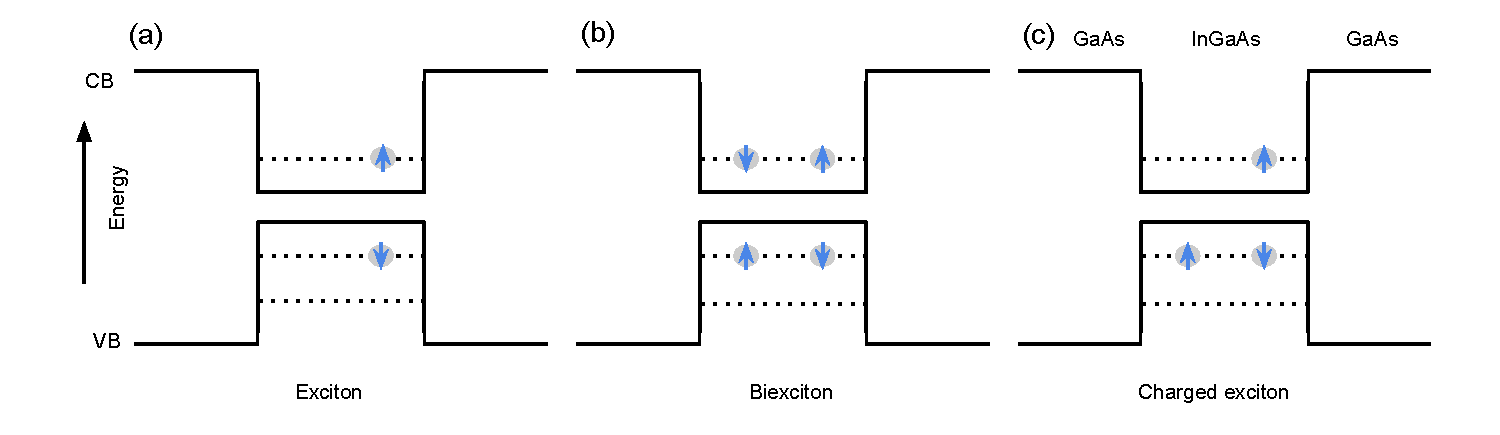
\includegraphics[width=1\textwidth]{images/estructure.pdf} \end{center}
\caption{Electronic structure of a quantum dot. (a) An exciton e-h pair. (b) A
biexciton with two e-h pairs. (c) An exciton with an extra hole making a
positively charged exciton.} \label{fig:estructure} \end{figure}

The discrete energy levels in the QD give rise to clean, sharp emission lines.
There is a well defined energy for each transition and as such the emitted
photons have a well defined wavelength, limited by the lifetime of the state.

\subsection{Single photon emission from Quantum dots }

The angular momentum of an electron is $\pm 1/2$ and for a hole is $\pm 3/2$.
The e-h pair can combine to make a state with spin $\pm 1$ for photon emission
and $\pm 2$ for nonradiative recombination. The energy of the emitted photon
corresponds to the energy of its original excitonic state. Thus the emitted
photons can be spectrally filtered to analyse the emission from only one
excitonic state.

\begin{figure}[h!] \begin{center}
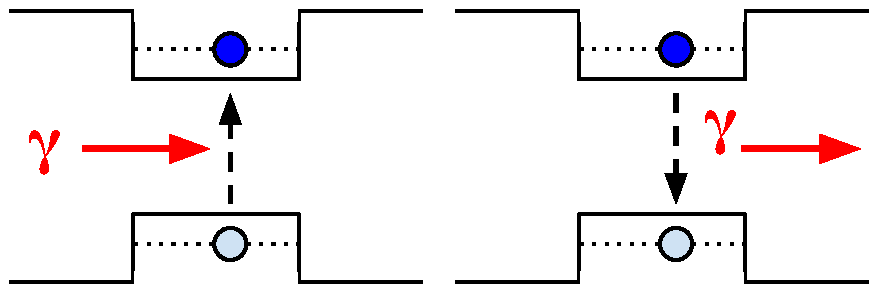
\includegraphics[width=1\textwidth]{images/qd_photon.pdf} \end{center}
\caption{Single photon emission process in a quantum dot.} \label{fig:qd_photon}
\end{figure}

For a light source with Poissonian emission statistics such as a laser true
single photon emission can not be achieved even with significant attenuation
because the probaility for multi photon emission still exists. In the case of a
quantum dot since each excitonic energy level can only accept a fixed number of
carriers and after photon emission there is a finite time which must pass before
more carriers can be captured true single photon emission is possible. This
process is shown schematically in Figure \ref{fig:qd_photon}. This single photon
emission can be verified by measuring the two photon second order correlation
function \begin{equation} g^{(2)}(\tau) = \frac{\left\langle I(t)I(t+\tau)
\right\rangle}{\left\langle I(t) \right\rangle \left\langle I(t+\tau)
\right\rangle} \end{equation} This is done by doing a Hanbury Brown Twiss
measurement. A stream of single photons impinge on a 50:50 beamsplitter. The two
outputs of the beamsplitters are sent to single photon detectors. One of the
detector signals is delayed by a time $\tau$ in order to measure both positive
and negative correlation times. If the source is a true single photon source
there will be a lack of coincidence clicks on both detectors when $\tau = 0$,
and thus $g^{(2)}(0)$ will be zero. Single photon emission from QDs has been
demonstrated under a wide range of excitation conditions - DC and AC electrical
excitation, continous wave (cw) and pulsed lasers at above band, quasi-resonant
and resonant energies.

\section{Semiconductor waveguides}

A dielectric waveguide is a core material surrounded by a material of lower
refractive index. The surrounding material is known as the waveguide cladding.
Here the theory is set out as in Integrated Photonics by Saleh and Teich
\cite{saleh1991fundamentals}. As an introduction to the design of waveguides in
this section the propogation of light in a symmetric dielectric slab waveguide
will be discussed. A core slab of refractive index $n_1$ is clad by two slabs of
refractive index $n_2$. This structure is shown in Figure
\ref{fig:planar_reflection}. The critical angle for the total internal
reflection of light is derived from Snells law to be

\begin{equation} \theta_c = \arcsin{\frac{n_1}{n_2}}. \end{equation}

When light impinges on the boundary of $n_1$ and $n_2$ with an angle less than
$\theta_c$ then it is reflected. Figure \ref{fig:planar_reflection} shows a
guided and unguided ray of light. The unguided ray hits the boundary with an
angle greater than $\theta_c$ and therefore some of the light refracts,
therefore losing some of the light at each reflection causing the ray to
eventually vanish. The guided ray hits the boundary at an angle less than
$\theta_c$ and reflects without any loss of power and will propagate along the
core.

\begin{figure}[h!] \begin{center}
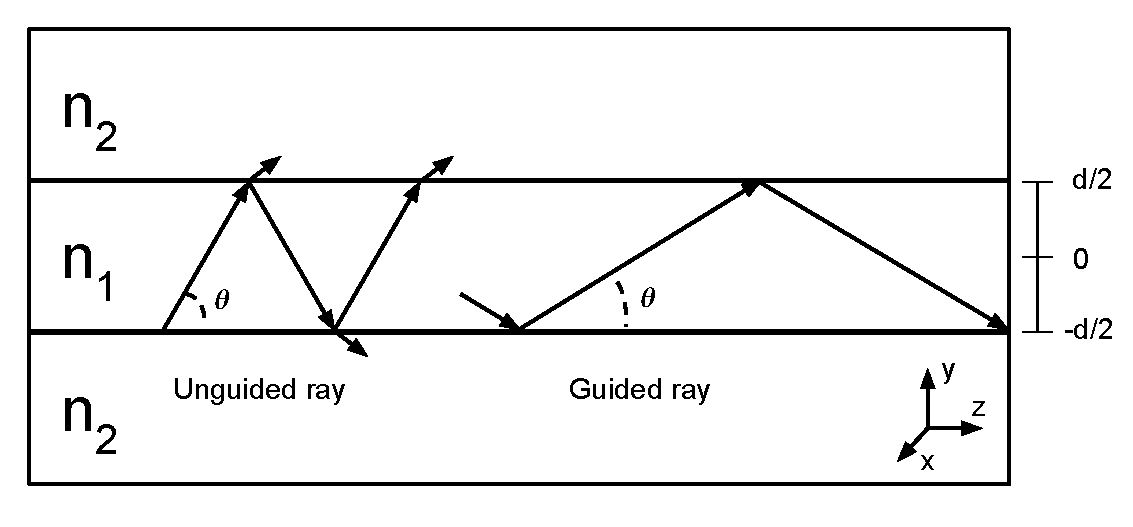
\includegraphics[width=0.8\textwidth]{images/thesis_planar_reflection.pdf}
\end{center} \caption{Light ray propagation in a planar dielectric waveguide.}
\label{fig:planar_reflection} \end{figure}

To understand the waveguide modes in the structure assume there is a transverse
electromagnetic (TEM) plane wave propogating in the waveguide core. This TEM
wave has a wavelength $\lambda = \lambda_0/n_1$ where $\lambda_0$ is the free
space wavelength. The wave is reflecting each time at the boundary with an angle
less than $\theta_c$ so the wave propagates in the core without loss of power.
With each reflection the wave lags behind the original by a distance
$2d\sin{\theta}$ \cite{saleh1991fundamentals}. There is also a phase $\phi_r$
change induced by each internal reflection. There is now a self-consistancy
condition imposed upon the reflected wave. As the wave reflects twice it
reproduces itself, waves which satisfy this condidion are known as eigenmodes,
or modes of the waveguide. The wave interferes with itself a pattern is created
which does not change with $\hat{z}$. Due to this self-consistency the phase
shift between the waves is zero or a multiple of $2\pi$, giving rise to the
condition

\begin{equation}\label{eqn:mode_eqn} 2 k_y d - 2 \phi_r = 2\pi m, \ \ \ \ m =
\mathrm{0, 1, 2,...} \end{equation}

where $k_y = n_1 k_0 \sin{\theta}$. The phase shift $\phi_r$ in the transverse
electric (TE) case due to total internal reflection is given by

\begin{equation} \tan{\frac{\phi_r}{2}} =
\sqrt{\frac{\sin^2\theta_c}{\sin^2\theta} - 1}. \end{equation}

Combining this with Equation \ref{eqn:mode_eqn} it is deduced that

\begin{equation}\label{eqn:trans} \tan \left( \pi \frac{d}{\lambda} \sin \theta -
m \frac{\pi}{2} \right) = \sqrt{\frac{\sin^2\theta_c}{\sin^2\theta} - 1}
\end{equation}

\begin{figure}[h!] \begin{center}
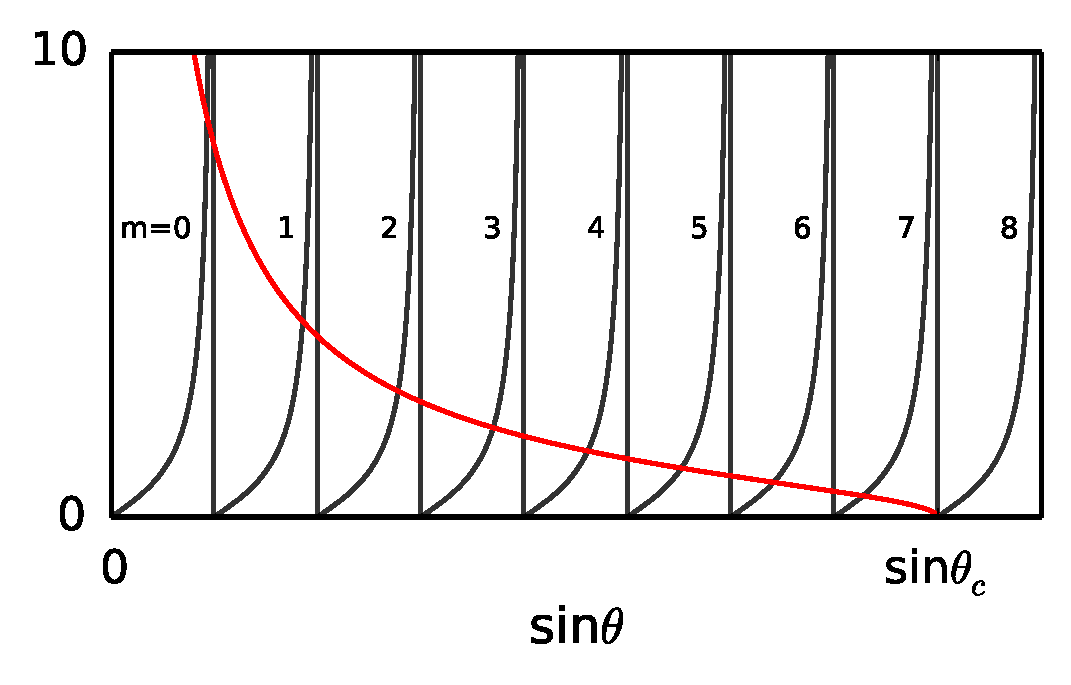
\includegraphics[width=0.8\textwidth]{images/mode.pdf} \end{center}
\caption{Graphical solution of Equation \ref{eqn:trans}. The black line is the
LHS of the equation and the red line is the RHS. Each LHS segment corresponds to
a mode in the waveguide.} \label{fig:mode} \end{figure}

This equation is trancendental and can be solved graphically, this solution is
shown in Figure \ref{fig:mode}. The LHS is a set of tan, when $m$ is even, and
cot functions, when $m$ is odd. Each LHS segment corresponds to a mode in the
waveguide. When the LHS crosses the x-axis, indicated by the semicircles, $\sin
\theta_m$ can be determined. The distance between these intersections is
$\lambda/2d$. The solution for transverse magnetic (TM) is very similar, with
just a different phase change upon reflection $\phi_r$. This information can be
used to deduce how many TE modes are in a waveguide of a given size $d$. The
number of modes M is given by the amount of segments of width $\lambda/2d$ exist
before $\sin \theta$ reaches the value $\sin \theta_c$.

\begin{equation}\label{eqn:nummodes} M = \frac{\sin \theta_c}{ \lambda / 2d},
\end{equation}

rounded up to the nearest integer. By substituting $\cos \theta_c = n_2/n_1$
into Equation \ref{eqn:nummodes} it is seen that

\begin{equation}\label{eqn:nummodes} M = 2\frac{d}{\lambda} \mathrm{NA}
\end{equation}

where

\begin{equation} \mathrm{NA} = \sqrt{n_1^2-n_2^2} \end{equation} is the
numerical aperture of the waveguide. The $\mathrm{NA}$ defines the range of
angle from which the waveguide can collect light. Equation \label{eqn:nummodes}
is extremely important in waveguide design because it defines the single-mode
cutoff for when $M \leq 1$. This impacts the choice of $d$ and the wavelength
for which the waveguide is single mode or multimode. Single mode waveguides are
generally more useful for quantum optics because they allow two photon
interference between light coming in from two single mode channels, this allows
the operation of directional couplers and Mach Zehnder interferometers. Single
mode optical fibres have lower loss in the telecommunications wavelength ranges
so is better suited to long distance communication.

\subsection{Two dimensional waveguides}

\begin{figure}[h!] \begin{center}
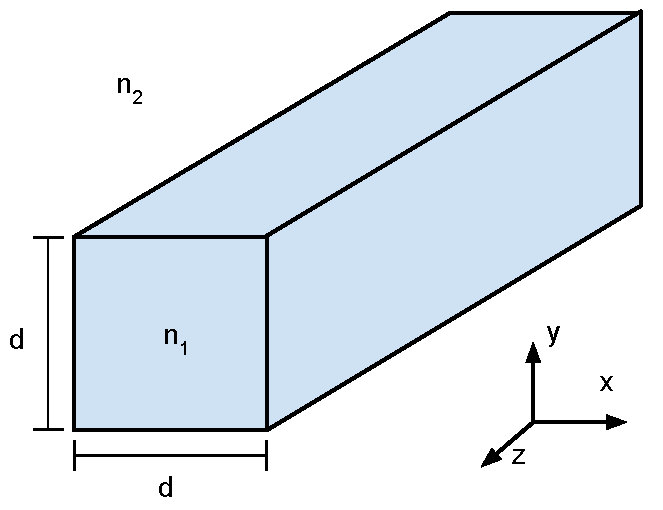
\includegraphics[width=0.5\textwidth]{images/2d_waveguide.pdf} \end{center}
\caption{Index structure of a waveguide which confines light in two dimensions.
The light is confined in $\hat{x}$ and $\hat{y}$ but is free to propagate in the
$\hat{z}$ direction.} \label{fig:2dwg} \end{figure}

A two dimensional dielectric waveguide is one which confines light along two
axes and allows the light to free  propagate along the third axis. A schematic
of a rectangular waveguide is shown in Figure \ref{fig:2dwg}. The modes and
number of modes can be derived in a similar fashion as for the planar dielectric
waveguide and shall just be quoted here \cite{saleh1991fundamentals}. The number
of modes in a two dimensional waveguide can be approximated by

\begin{equation} M \approx \frac{\pi}{4} \left( \frac{2d}{\lambda_o } \right)^2
\mathrm{NA}^2. \end{equation}

This approximation holds well for multimode waveguides, but loses accuracy near
the single mode boundary. Design of single mode two dimensional waveguides
generally needs to be solved computationally.

\subsection{Directional couplers and Mach Zehnder interferometers}

\begin{figure}[h!] \begin{center}
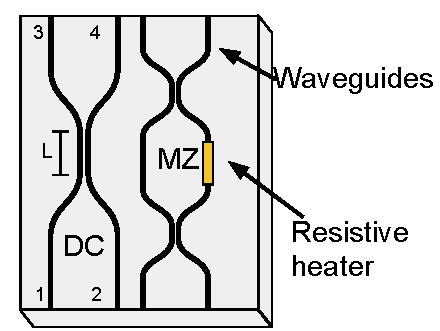
\includegraphics[width=0.7\textwidth]{images/wg_devices.pdf} \end{center}
\caption{Two common waveguide devices, a directional coupler and a Mach Zehnder
interferometer. The numbers on the directional couplers indicate input and
output ports which shall be reference in the text, equivalent ports shall be
used for the Mach Zehnder interferometer.} \label{fig:wg_devices} \end{figure}

Figure \ref{fig:wg_devices} shows the schematic of two waveguide devices used
frequently throughout this project. A directional coupler (DC) is a photonic
device which splits the power between two output ports with a well defined
coupling ratio between the ports. Two waveguides are brought close enough so
that the evanescent fields overlap. The waveguides are assumed to be single
mode. It can be derived that the power in each port 3 and 4 in Figure
\ref{fig:wg_devices} as a result of light of power $P_1$ being injected to the
coupler from port 1 is

\begin{equation} P_3(z) = P_1 \cos^2 cz \end{equation} \begin{equation} P_4(z) =
P_1 \sin^2 cz \end{equation}

Where $z$ is the propagation direction and $c$ is the coupling coefficient
related to the index contrast of the waveguide, the separation $d$ between the
waveguides in the interaction region and the operating wavelength.

A Mach Zehnder interferometer (MZI) is a sequence of two DCs in parallel. The
light splits 50/50 into two arms by the first DC. On one of the arms is a local
refractive index changing element, this can be a electrode to take advantage of
the electro-optic effect or heater, for the thermo-optic effect. Here it shall
be assumed to be a heater. This element changes the local refractive index in
the arms. This causes a phase mismatch between the light propagating in each arm
so that the light will constructively or destructively interfere at the second
DC. By tuning the heater this phase can be chosen an light can be arbitrarily
coupled between ports 3 and 4. This is called a Mach Zehnder interferometer
switch or modulator. These are used extensively in telecommunications to route
signals between different channels.

 \section{Integrated quantum devices}

Semiconductor quantum dots and waveguides are interesting technologies on their
own. However this thesis focuses on the combination of these technologies to
create a platform capable of making working integrated quantum devices in the
future.

In the approach of these thesis laid out in Chapter 2 and 3, we attach a QD
filled GaAs chip to the end of a SiON based photonic circuit. This approach
allows us to make custom designed photonic circuits, which are fabricated
seperately from the QD quantum light source. The circuits are made up of a
series of MZI's. This thesis focuses on the initial fabrication and
demonstration of the platform. In the next phase of reseach there are many
target circuits which are interesting for quantum telecommunications which have
been demonstrated with QD's with bulk optics, but not yet reproduced on an
integrated device. CNOT gates\cite{cnotpooley}, quantum relays'
\cite{varnava2015entangled}, quantum amplifiers \cite{kocsis2013heralded,
zavatta2011high}, NOON state generations \cite{bennett2015cavity} and various
combiners and splitters.

\subsection{NOON states and quantum sensing}

This section will describe a useful application of quantum sources and quantum
circuits, generating a NOON state. The dynamics of a NOON state as is passed
through a MZI allow it to be super sensitive to phase changes in the MZI.
A NOON state is a many particle quantum entangled state. It is represented as:

\begin{equation} \left|\psi\right\rangle = \left|N\right\rangle_{a}
\left|0\right\rangle_{b} + e^{iN\theta} \left|0\right\rangle_{a}
\left|N\right\rangle_{b} \end{equation}

this state is a superposition of $N$ particles in mode $a$ and 0 particles in
mode $b$ and vica-versa. The particles need to be bosonic and in this case the
quantum particles are photons.

To generate this state using photonics we consider the state generated by
photons propagating through an MZI. In the single photon case, single-photon
interference occurs from the path length difference in the two arms of the MZI.
One of the photon modes gathers a phase shift $\Delta \phi$ and causes the
detection probabilities of the MZI output arms to change.

The probabilities become $P_1 = 1 + \cos{\Delta \phi}$ and $P_2 = 1 +
\sin{\Delta \phi}$.

This interference is generalised by Hong-Ou-Mandel interence \cite{hongoumandel}
for multiple photons. The biphoton state must then be represented by a path
entangled state:

\begin{equation} \left|\psi\right\rangle = \left|2\right\rangle_{a}
\left|0\right\rangle_{b} + e^{i2\theta} \left|0\right\rangle_{a}
\left|2\right\rangle_{b} \end{equation}

In this case the oscillation of the detection probabilities depending on phase
is twice as fast. $P_{1, 1} = 1 + \cos{2 \Delta \phi}$ and $P_{2, 2} = 1 +
\sin{2 \Delta \phi}$.

This path encoded biphoton state is the same a two particle NOON state. It is
seen that the phase modulation increases linearly with the number of particles
in the state $N\Delta \phi$. This would allow smaller phase changes to be
detected faster by some quantum sensor, this is known as superresolution.

It can also be seen that the error in the phase measurement becomes smaller for
larger $N$. Consider the observable

\begin{equation} O = \left|N, 0\right\rangle \left\langle 0, N\right| + \left|0,
N\right\rangle \left\langle N, 0\right| \end{equation}

The error in the phase becomes

\begin{equation} \Delta \phi = \frac{\Delta O}{ | d \left\langle O \right\rangle /
d \phi | } = \frac{1}{N} \end{equation}

Thus the phase error decreases with increasing particle number, this is known as
supersensitivity.

NOON state super resolution can be achieved experimentally using quantum dots
and an integrated photonic circuit \cite{bennett2015cavity}. QDs are resonantly
excited in order to achieve long coherence times and good two photon
interference visibilities.

The photons are generated sequentially from the QD, they are directed to a 50:50
beamsplitter where one are is delayed. This causes 25% of the sequential photons
to be time synched in parallell.

The two photons are then sent into a MZI, whereby detecting the coincidences
from the outputs the phase of the MZI can be determined accurately.

In an integrated photonic circuit MZI, the phase of one arm is changed by
inducing a refractive index change on that arm. This refractive index change
causes a change in the phase of the circuit. This phase change is then measured
with high sensitivity by the NOON state, allowing a supersensitive measurement
of whatever caused the refractive index change.

Any component which changes the refractive index of one arm can then be sensed.

For example, placing a conducting gold strip over one arm will induce a refractive
index change when there is a current run through the strip. This current can then be
supersensed.

If a microfluidic channel is placed in the path of the light going down one arm of
the MZI, the fluid will have a different refractive index depending on its contents.
This can be used to sense trace amounts of components inside the fluid \cite{crespi2012measuring}.
